\title{\textbf{Christian perspectives on sustainability: \\
		The need for numerical answers to philosophical questions.}}
% Sustainability challenges and managing tradeoffs: engineers' need for numerical answers to philosophical questions 
\author{
		% Authors must be italicized.
        \emph{Jeremy Van Antwerp} and \emph{Matthew Kuperus Heun}%
\footnote{
Engineering Department, 
Calvin College,
Grand Rapids, MI, 49546, USA}
}

\documentclass[12pt]{article}

% CEC papers should be set in Times New Roman.
% https://tex.stackexchange.com/questions/153168/how-to-set-document-font-to-times-new-roman-by-command
% suggests the following.
\usepackage{mathptmx}             % For Times New Roman font (or a close approximation thereof).
\usepackage[margin=1in]{geometry} % For 1-inch margins all around.
\usepackage[document]{ragged2e}   % For left justification.
\usepackage{parskip}              % For double-spacing between paragraphs.
\usepackage{nopageno}             % To eliminate page numbers.
% For MLA bibliography. See https://www.ctan.org/pkg/biblatex-mla?lang=en for details.
\usepackage[american]{babel}
\usepackage{csquotes}
\usepackage[style=mla-new]{biblatex}
\addbibresource{JVAMKH.bib}
\usepackage[inline]{enumitem}  % For inline enumerate* lists

\usepackage{titlesec}             % To change formats of section titles, etc.
\titleformat*{\section}{\normalsize}
\titleformat*{\subsection}{\normalsize}
\titleformat*{\subsubsection}{\normalsize}
\titleformat*{\paragraph}{\itshape} % Set paragraph titles to italics
\usepackage{abstract}             % Set characteristics of the abstract
\setlength{\absleftindent}{0in}   % Do not indent left side
\setlength{\absrightindent}{0in}  % Do not indent right side
\usepackage{url}
\setlength{\parindent}{0in}       % Do not indent the 1st line of paragraphs.
\setlength{\parskip}{12pt}        % Instead, add space between paragraphs.
\renewcommand{\abstractnamefont}{\normalfont\normalsize} % Unbold and regular size
\renewcommand{\abstracttextfont}{\normalfont\normalsize} % Unbold and regular size
\date{}                           % To eliminate the date in the title

% To include graphics
\usepackage{graphicx}

% Commands for editing.

\usepackage{xcolor}            % For colored text
\usepackage[normalem]{ulem}    % For \sout command (strikethrough)

% From https://tex.stackexchange.com/questions/130623/crossing-out-using-different-colour,
% Change the \sout color to red
\newcommand{\redsout}{\bgroup\markoverwith{\textcolor{red}{\rule[0.5ex]{2pt}{0.4pt}}}\ULon}

% Use these versions to display changes.
\newcommand{\del}[1]{\textcolor{gray}{\redsout{#1}}}
\newcommand{\ins}[1]{\textcolor{red}{#1}}
\newcommand{\rev}[2]{\del{#1}\ins{#2}}

% Use these versions for a clean copy.
% \newcommand{\del}[1]{}
% \newcommand{\ins}[1]{#1}
% \newcommand{\rev}[2]{#2}



\begin{document}
	
\maketitle

\begin{abstract}
\noindent
\ins{rewrite abstract from scratch. Later.}

\end{abstract}


%%%%%%%%%%%%%%%%%%%%%%%%%%%%%%%%%%%%%%%%%%%%%%%%%%%%%%%%%%%%%%
\section{Sustainability and the disciplines}
\label{sec:sustainability_and_the_disciplines}
%%%%%%%%%%%%%%%%%%%%%%%%%%%%%%%%%%%%%%%%%%%%%%%%%%%%%%%%%%%%%%

Sustainability is challenging because of complexity, scales humans are ill-suited to consider, 
and lack of helpful philosophical and theological frameworks.

Because of circumstances in our world today, 
concerns about environmental, economic, and social 
issues are significant. 
The concept of ``sustainability'' encompasses all three areas
with a view toward the future. 
(See Figure~\ref{fig:3_sustain}.)
One definition of sustainability is
``Sustainability emerges from choices that, on balance, 
promote economic vitality, social equity, and a flourishing natural environment 
both now and for generations to come''~\autocite{Calvin-College-2017}.

Sustainability is considered to be a ``grand challenge,'' 
and becoming more sustainable requires solving 
complex, multidisciplinary, and multifaceted problems
with both technical and non-technical, even philosophical, aspects. 
We engineers design and operate the machines and systems that
%
\begin{enumerate*}[label={(\alph*)}]

  \item generate economic growth by providing employment and economic output, 

  \item enhance society bring people together through communication technologies, and
        
  \item enhance the natural environment.

\end{enumerate*}
%
But we also design machines and systems that
%
\begin{enumerate*}[label={(\alph*)}]

  \item replace human workers,

  \item foster online hate, and
        
  \item consume non-renewable materials and
        emit pollution, thereby contributing to environmental degradation.

\end{enumerate*}
%
Which direction a particular machine or system propels society is a function, in part,
of both its design and of the macro socio-economic policies that inform the design.
Because design is a central function of engineering, 
engineers have an important role to play in determining 
the sustainability of our future. 

But what guides engineers to make design choices that lead to sustainability?
And what guides policy-makers to make socio-economic-environmental
policy choices from which sustainability can emerge?

A traditional answer is ``the academic disciplines,'' 
which are both generators of and repositories for accumulated human knowledge
about a problem domain.
Presumably, academic disciplines can guide design processes for engineers
and policy-making for policy-makers.
Of course, there are academic disciplines 
at each vertex of the sustainability triangle (Figure~\ref{fig:3_sustain}):
Environmental Studies (or Ecology, Biology, etc.) for the Environmental vertex, 
Economics for the Economy vertex, and 
Sociology for the Social vertex.
But sustainability grand challenges exist across disciplinary boundaries and, by definition,
cannot be addressed or solved by a single vertex discipline alone.

\begin{figure}
\centering
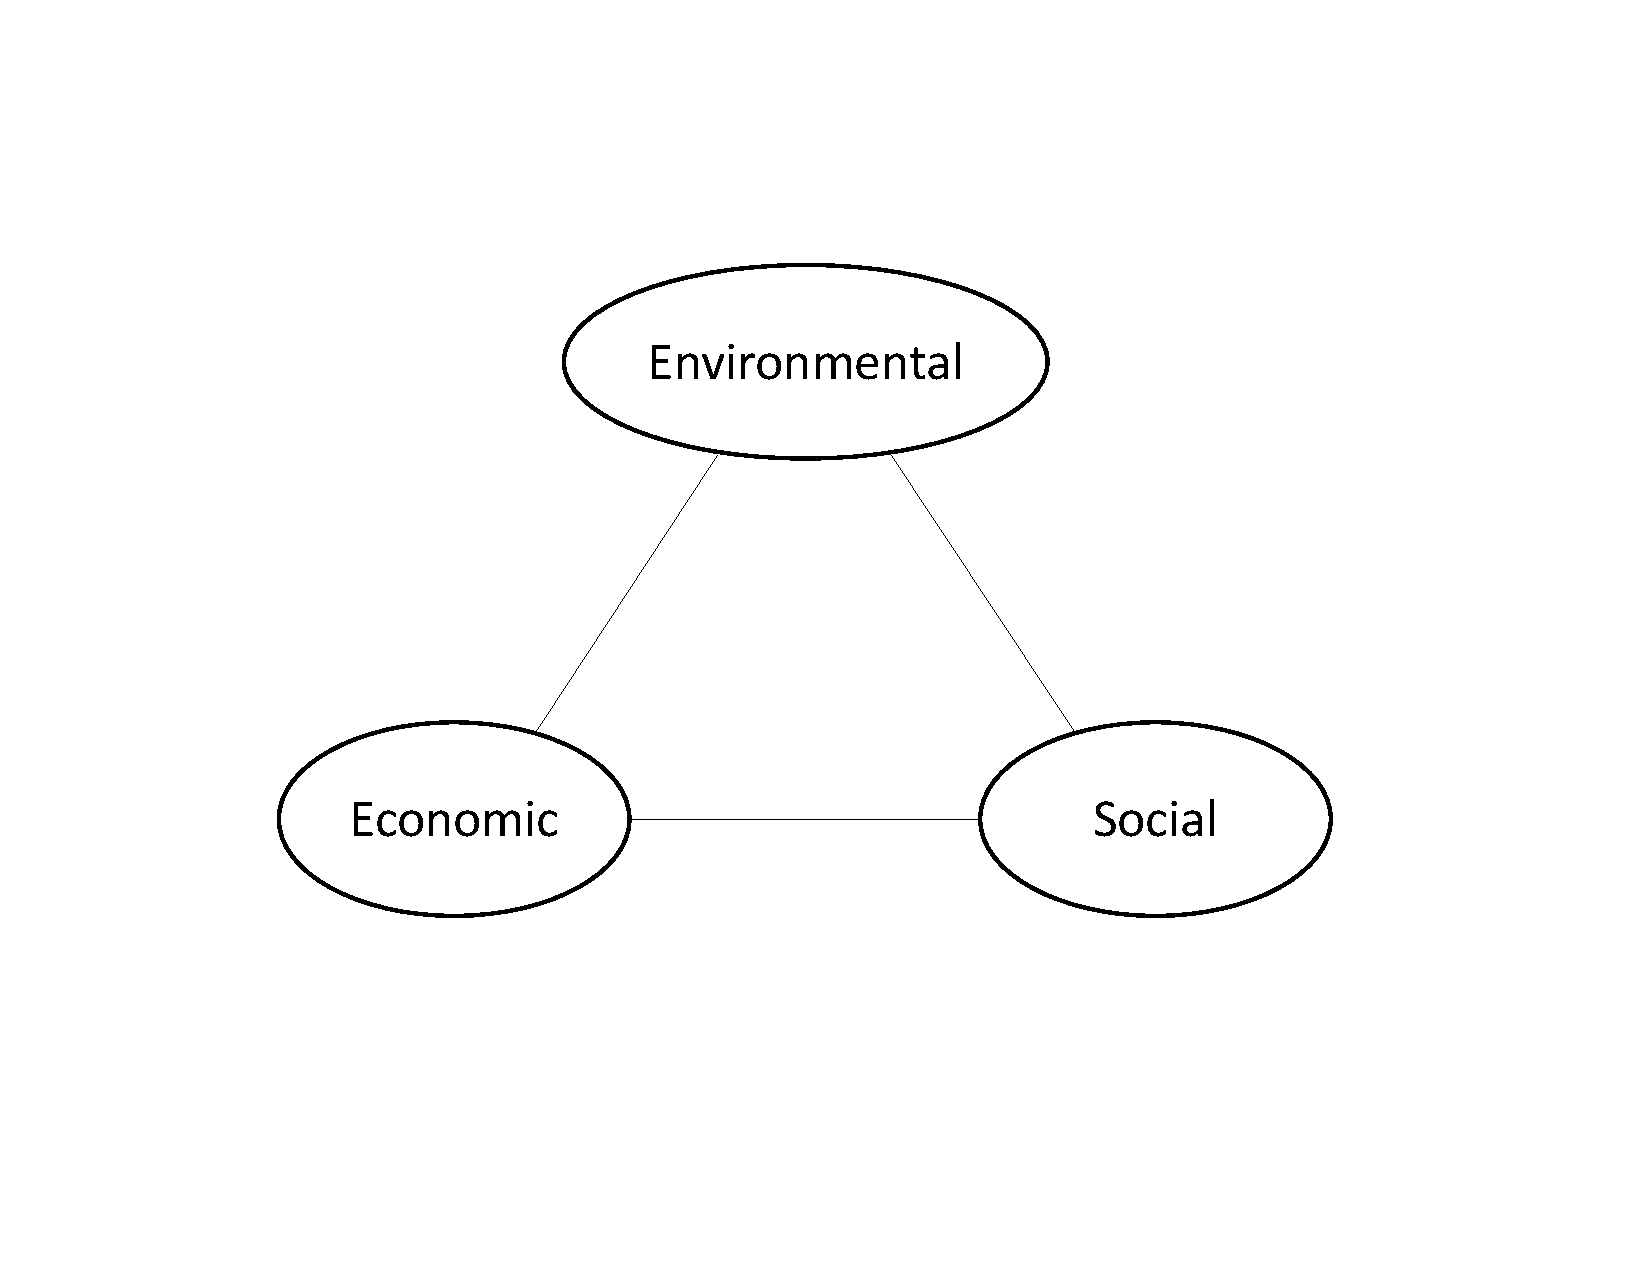
\includegraphics[width=0.75\linewidth]{figure_other/TriangleDiagram.pdf}
\caption{Three aspects of sustainability.}
\label{fig:3_sustain}
\end{figure}

In a hopeful interdisciplinary sign, 
disciplines have emerged along the edges of Figure~\ref{fig:3_sustain}, too.
Environmental Economics was founded in the 1960s,
focusing on valuation of ecosystem services and 
internalizing externalities associated with environmental degradation.
In the 1970s, Environmental Sociology emerged along the Environmental--Social edge 
to study interactions between society and the natural environment. 
Along the Social--Economics edge, Socioeconomics (also called Social Economics) 
emerged in the early 1980s
to study interactions between societies and their economies.
Ecological Economics, founded in the late 1980s, 
emphasizes that the economy as a subsystem of the environment.
There are journals for each edge:
the \emph{Journal of Environmental Economics and Management}, \emph{Ecological Economics}, 
\emph{Environmental Sociology}, 
the \emph{International Journal of Social Economics}, and the \emph{Journal of Socio-Economics}.

However, our assessment of the vertex and edge disciplines,
as presently constituted,
is that they are not policy-relevant
at the macro level. 
For example, these disciplines would focus on the best way to manage a particular forest 
rather than the best way to preserve forests worldwide
in the context of broad economic and social factors.
Furthermore, these edge disciplines exist, almost by definition, 
on the fringes of the vertex disciplines:
E.g., Ecological Economics is not considered ``real'' economics by many economists.
The edge disciplines, by and large, do little to affect the vertex disciplines.

Additionally, what guides Christian engineers to make sustainable design choices
that glorify God and serve humankind
or policy-makers to generate policies that do the same?
One might think that ``Christian Theology'' could provide answers, because
one aspect of theology is discerning the 
ways that deities interact with the natural world. 
However, most Christian thought is focused on interactions among people 
and between individuals and divine beings.

It is rare for Christian theologians to grapple seriously with 
sustainability issues.
We have yet to see sustainability issues engaged in a serious and widespread manner
by Christian theologians and scholars or by denominations.
Thus, to date, there is little indication that Christian Theology 
has provided helpful guidance on sustainability issues
for engineers or policy-makers.


There has been a lot of work in the area of sustainability, but most of it is flawed in one or more ways.
Sometimes sustainability \emph{is} a zero-sum game 
(for instance, you can't \emph{both} use fossil fuels and conserve fossil fuels)
and sometimes sustainability \emph{isn't} a zero-sum game 
(technical innovation sometimes can both improve standard of living and be more energy efficient).
Much of the literature on sustainability assumes that it is possible to have both ``development,'' by which it is meant lifting people out of poverty,
and environmental conservation. 
For example, ``Humanity has the ability to make development sustainable ... widespread poverty is no
longer inevitable if policies that nurture and favor growth are adopted and implemented'' \cite{Ngome2015}.
However, prosperity and conservation are generally at odds. Economic activity requires input of resources
and produces outputs such as pollution. Fundamentally, economic growth is itself unsustainable; at some level of economic activity,
the Earth will not be able to supply the inputs needed and/or absorb the outputs humans produce.

Another common error in the sustainability literature is the assumption that it will be possible to move 
from our current situation to a sustainable future. These studies look forward to an ideal future state without
serious consideration of whether a sustainable future state is practically, physically, and/or technically achievable. 
One helpful question to discern fanciful or wishful thinking in this regards is ``what would have to be true for this to happen?''
For example, it is generally understood that a carbon-neutral energy sector is necessary for sustainability.
What would have to be true for the world to transition to an energy sector that doesn't emit greenhouse gases?
\begin{itemize}
\item There would have to be massive investments in renewable-energy generation. 
Replacing all coal-fired power plants in the United States (1.2 trillion kW-hrs/yr) %citations needed.
with solar generation would require about 4 million acres of land 
(about 0.2\% of the US land area, or about half the state of Maryland) 
and an investment of $2 trillion, which is about one tenth of the annual US GDP.
\item There would have to be massive energy storage. Eighteen to 40 hours worth of electricity storage would 
have been needed for a fully renewable grid to get the Midwest and Northeast through the January 27 -- February 2, 2019 polar vortex.
\item There would have to be massive changes to the electricity distribution grid.
\item There would be massive disruptions to large sectors of the economy. 
Oil and gas exploration and extraction would be almost entirely diminished.
Gas stations would be out of business -- or maybe changed to charging stations.
\end{itemize}


%%%%%%%%%%%%%%%%%%%%%%%%%%%%%%%%%%%%%%%%%%%%%%%%%%%%%%%%%%%%%%
\section{Questions}
\label{sec:questions}
%%%%%%%%%%%%%%%%%%%%%%%%%%%%%%%%%%%%%%%%%%%%%%%%%%%%%%%%%%%%%%

\ins{flow from questions to gaps in how Christians think about sustainability.}
Each paragraph ends with a question (in italics) 
move the the ends of motivating question ==> We lack tools to give concrete answers to these questions.

\subsection{Social}
For any given level of technological development, there must exist some upper limit to the human population the Earth
can support. Calculating this limit is a technical question and can be technically addressed. The subsequent questions are nontechnical.
\begin{itemize}
\item ``What is the ideal total population?'' (which is less than or equal to maximum possible population) % informed by environmental (and economic?) tradeoffs.
\item ``How should we manage for and arrive at this ideal population?'' and % a means/ends question.
\item ``Where should people live? What is the geographical distribution of population?'' % rights, standard of living = justice.
\end{itemize}
Answers to these questions depend a great deal on \emph{values}. What are the relative preferences for justice, standard of living, 
environmental versus economic and social tradeoffs, and the relative importance of the means versus the end?

What ``right'' do people have to food, water, air, medicine or health care, property, or a ``living'' wage? 
Where do these rights come from? What rights does the nonhuman world have? Where do these rights come from?
What rights do future generations have, and where do their rights come from? % love your neighbor as yourself?
When tradeoffs exists between these rights, how do we manage resolution?
How do/should Christian assessments of tradeoffs change when cost and benefits fall to different (groups of) people?
Does it depend on whether many benefit at the expense of a few of if few benefit at the expense of many? 
When benefits and costs accrue to different generations? 
Does the size of the benefit/cost matter? 
Does the number of people in the group matter? Surely, it must but what is a ``large enough'' difference to matter?

Regarding gloomy predictions about sustainability issues, such as climate change, global population,
or in terms of world energy supply, there are those who will say ``don't worry, it will all work out,'' while
others respond ``no it won't.'' Who should we give credence to? Obviously, those who are telling the truth. But that can
be hard to identify. (The Old Testament criteria for determining the legitimacy of a prophet comes to mind, but the
Israelites had a poor track record of following prophetic advice.) There are technical truths and moral truths. Should
the opinion of an expert researcher or technologist count for more than a blue-collar ``man on the street?'' How about a
government leader? Does it matter if the question under consideration is technical or nontechnical?

\subsection{Social economics}

A policy-driven change, such as reducing carbon emissions by banning air travel, results in consequences that have
\emph{direct} dollar-measurable impacts (such as change in GDP), \emph{indirect} but still dollar-measurable
consequences (such as reduced CO$_2$ output), and consequences that \emph{aren't} measurable in dollars (such as an
aesthetic impact on the landscape). Economic cost-benefit analysis converts all social and environmental costs to
dollars, thereby providing a consistent numeraire and allowing direct comparisons among environmental, economic, and
social effects. How should Christians evaluate choices among policy solutions whose impacts are dollar-quantifiable and
those that are \emph{not} dollar-quantifiable? 

\subsection{Environmental social justice}
How do Christians balance stewardship of the natural world with loving our neighbor?
Both the Old and New Testaments teach that Christians should work to eliminate poverty. 
How do we respond to the observation that alleviating poverty increases economic consumption, which has negative environmental consequences?
Suppose a third-world farmer argues that he/she needs to make a living. 
Can he/she create another subsistence farm via slash-and-burn agriculture in the rainforest?  
It could be argued that it is sinful \emph{not} to make use of a resource, such as coal or petroleum. 


\subsection{Environmental economics}
There are those who say that coal mining is good because the benefit of employment in the coal industry outweighs
any (potential) environmental harm caused from mining and burning coal. How large does the cost-benefit differential
have to be for this to be true? This is an entirely practical question that demands a concrete, numerical answer.

Some consequences of a ban on air travel would include the destruction of the air travel industry and its ancillary
industries. How does the weighing of tradeoffs (e.g., economic versus environmental) differ if the loss of jobs is not
the result of a regulation, but instead comes from technological innovation or market forces? Should this make a
difference? Does it?

\subsection{Multifaceted sustainability}
In 2013, air travel was responsible for about 3\% of US greenhouse gas emissions. % citation needed. EPA data appears to be offline now.
% see https://www.c2es.org/content/reducing-carbon-dioxide-emissions-from-aircraft/
% which cites Inventory of U.S. Greenhouse Gas Emissions and Sinks: 1990–2015 (U.S. Environmental Protection Agency, 2017)
Air travel is a particularly \emph{carbon intensive} activity. Therefore, banning air travel would be a step to making the 
world a more sustainable place. Engineers are well equipped to analyze some of the effects of this proposal. For instance,
engineers could estimate the resulting \emph{increase} in emissions from other forms of transportation that would result from 
the ban on air travel. However, \emph{how should the social and economic consequences be weighed against the environmental 
benefits}? What is the balance between the needs to the present and the needs of the future?	
Do economic, social, and environmental factors weigh differently in that decision?	

Banning air travel might be considered a ``clean'' or ``ideal'' policy option. Other policy options could be classified
as pragmatic, such as improving air travel energy efficiency. How should Christians navigate the space between ideal and
pragmatic policy proposals?



As a society, we have \emph{de facto} arrived at answers to questions such as the ones above. However, 
there is increasing reason to believe that the answers we have are not the answers that will lead to a sustainable future.
Moreover, the hows and whys of the answers that we have need to be reexamined.
\ins{Need a concluding and/or summarizing statement. Something along the lines of ``thus, it's clear that we lack the theological
and philosophical framework that would allow us to to address sustainability issues.''}

% Add: Utilitarian/Kantian ethics? Engineers like these because they allow us to calculate the greatest good for the greatest number of people.
% If an answer is mathematical, it must be true.


%%%%%%%%%%%%%%%%%%%%%%%%%%%%%%%%%%%%%%%%%%%%%%%%%%%%%%%%%%%%%%
\section{The need for a theology of sustainability}
\label{sec:need_for_theology_of_sustainability}
%%%%%%%%%%%%%%%%%%%%%%%%%%%%%%%%%%%%%%%%%%%%%%%%%%%%%%%%%%%%%%



%%%%%%%%%%%%%%%%%%%%%%%%%%%%%%%%%%%%%%%%%%%%%%%%%%%%%%%%%%%%%%
\section{Worldviews}
\label{sec:worldviews}
%%%%%%%%%%%%%%%%%%%%%%%%%%%%%%%%%%%%%%%%%%%%%%%%%%%%%%%%%%%%%%


% There has been a lot of work in the area of sustainability, but most of it is flawed in one or more ways.
% Sometimes sustainability \emph{is} a zero-sum game
% (for instance, you can't \emph{both} use fossil fuels and conserve fossil fuels)
% and sometimes sustainability \emph{isn't} a zero-sum game
% (technical innovation sometimes can both improve standard of living and be more energy efficient).
% Much of the literature on sustainability assumes that it is possible to have both ``development,'' by which it is meant lifting people out of poverty,
% and environmental conservation.
% For example, ``Humanity has the ability to make development sustainable ... widespread poverty is no
% longer inevitable if policies that nurture and favor growth are adopted and implemented'' \cite{Ngome2015}.
% However, prosperity and conservation are generally at odds. Economic activity requires input of resources
% and produces outputs such as pollution. Fundamentally, economic growth is itself unsustainable; at some level of economic activity,
% the Earth will not be able to supply the inputs needed and/or absorb the outputs humans produce.
%
% Another common error in the sustainability literature is the assumption that it will be possible to move
% from our current situation to a sustainable future. These studies look forward to an ideal future state without
% serious consideration of whether a sustainable future state is practically, physically, and/or technically achievable.
% One helpful question to discern fanciful or wishful thinking in this regards is ``what would have to be true for this to happen?''


%%%%%%%%%%%%%%%%%%%%%%%%%%%%%%%%%%%%%%%%%%%%%%%%%%%%%%%%%%%%%%
\section{Conclusions}
\label{sec:conclusions}
%%%%%%%%%%%%%%%%%%%%%%%%%%%%%%%%%%%%%%%%%%%%%%%%%%%%%%%%%%%%%%



\printbibliography
\end{document}